% HEADER
\documentclass[class=article, crop=false]{standalone}
\usepackage{00_Preamble/frr_preamble}

% Packages
\usepackage{titlesec}	
\usepackage{hyperref}
\usepackage{float}
\usepackage{graphics}
\usepackage{placeins}
\usepackage{adjustbox}
% END HEADER

\begin{document}
	\subsection{Layout}
	\label{subsec:payload_layout}
	\subsubsection{Full Assembly}
	The payload assembly is located in the fore section of the vehicle. As shown in Figure \ref{fig:360access}, the payload components are mounted along three threaded rods. These rods anchor into the SRC mechanism, connecting the payload to the vehicle. Payload components are attached to laser cut, 0.25" Baltic birch plywood shelves. Each shelf is customized in shape to meet the needs of its components, while maintaining at least three points of contact to the carbon fiber body tube. This allows every shelf to act as a centering bulkhead to prevent lateral movement of the payload.
	
	\bigbreak
	
	% \FloatBarrier
	% \begin{figure}[!h]
	% \captionsetup[subfigure]{justification=centering}
	% \centering
	% \begin{subfigure}{.45\textwidth}
	% \centering
	% \includegraphics[width=0.4\linewidth]{09_Figures/Payload/FullAssembly1.jpg}
	% \caption{CAD of full Payload Assembly}
	% \label{fig:payloadFullCAD}
	% \end{subfigure}
	% \begin{subfigure}{.45\textwidth}
	% \centering
	% \includegraphics[width=0.4\linewidth]{09_Figures/Payload/payloadOnSRC.png}
	% \caption{Payload with SRC and Camera Shrouds}
	% \label{fig:payloadOnSRC}
	% \end{subfigure}
	% \caption{CAD and Picture of Payload Assembly with SRC Mechanism and Camera Shrouds}
	% \label{fig:fullPayloadYeah}
	% \end{figure}
	% \FloatBarrier
	
	\FloatBarrier{}
	\begin{figure}[!h]
		\centering
		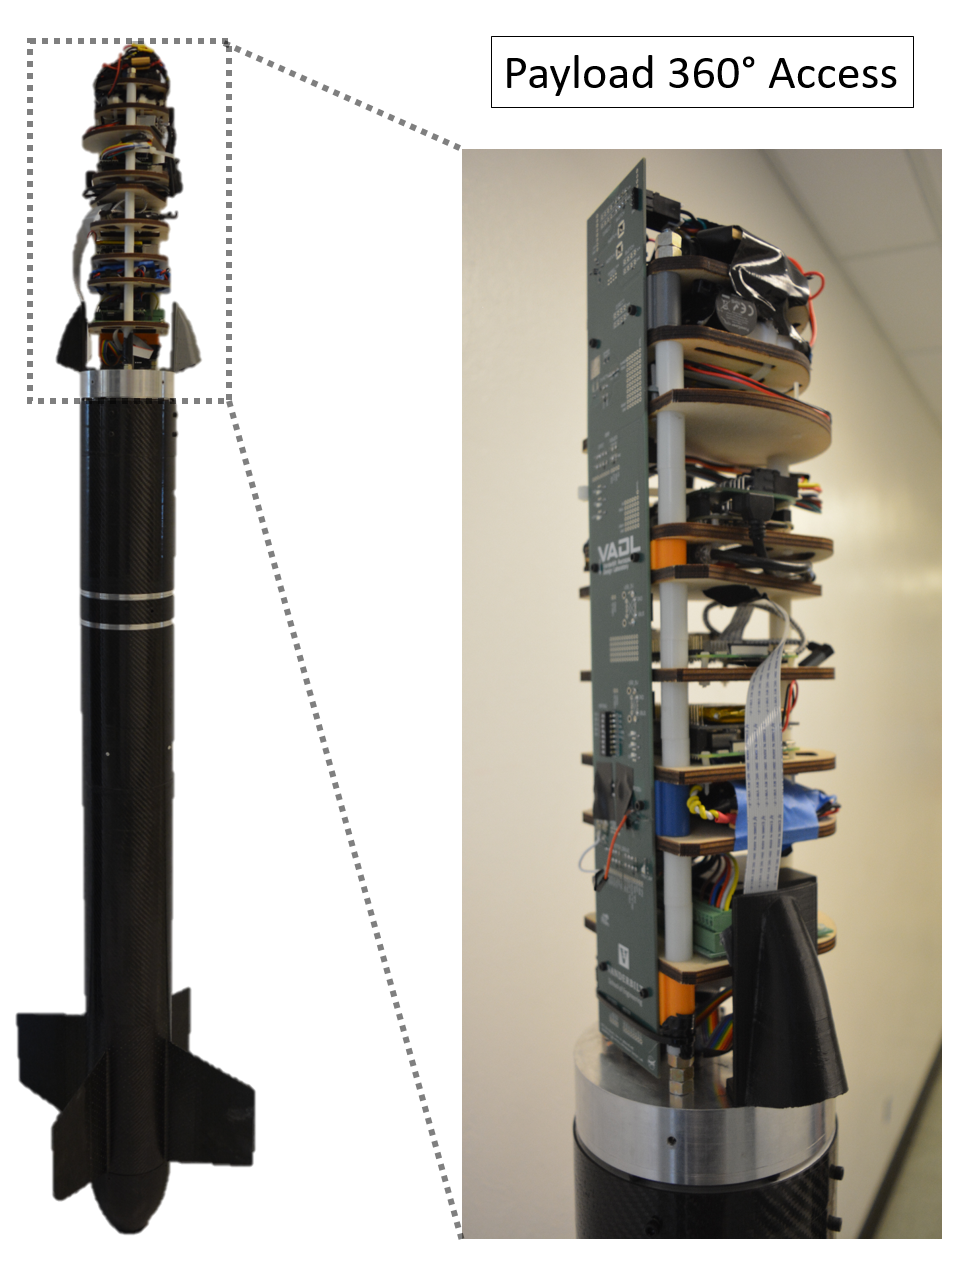
\includegraphics[width=0.7\linewidth]{09_Figures/Payload/360access.png}
		\caption{Flight-Ready Payload on Vehicle}
		\label{fig:360access}
	\end{figure}
	\FloatBarrier{}
	
	This physical layout offers a distinct advantage over the previous design in that it provides full access to all payload components and connections throughout assembly. As Figure \ref{fig:360access} illustrates, the launch vehicle with payload can reach the stage of full assembly before the nosecone and fore section carbon fiber tube are attached. This creates the opportunity to visually verify that all electrical and mechanical connections are satisfactory on the launchpad. Additionally, arming of payload power switches, experiment deployment over ethernet, and confirmation of status LEDs can be performed without any accessibility cut-outs in the vehicle body.
	
	% \FloatBarrier{}
	% \begin{figure}[!h]
	% \centering
	% \captionsetup{justification=centering}
	% \includegraphics[width=0.7\linewidth]{09_Figures/Payload/payloadFullOnLaunchpad.png}
	% \caption{Vehicle and Payload Configuration on Launchpad. \\ Design provides complete access to payload. \\ REPLACE WITH ACTUAL PHOTO!!!!!!!!!!!}
	% \label{fig:payloadFullOnLaunchpad}
	% \end{figure}
	% \FloatBarrier{}
	
	% Replaced by above figure with callout
%	\FloatBarrier
%	\begin{figure}[!h]
%		\captionsetup[subfigure]{justification=centering}
%		\centering
%		\begin{subfigure}{.58\textwidth}
%			\centering
%			\includegraphics[width=0.58\linewidth]{09_Figures/Payload/fullOnPadCAD.jpg}
%			\caption{CAD Model}
%			\label{fig:fullOnPadCAD}
%		\end{subfigure}
%		\begin{subfigure}{0.37\textwidth}
%			\centering
%			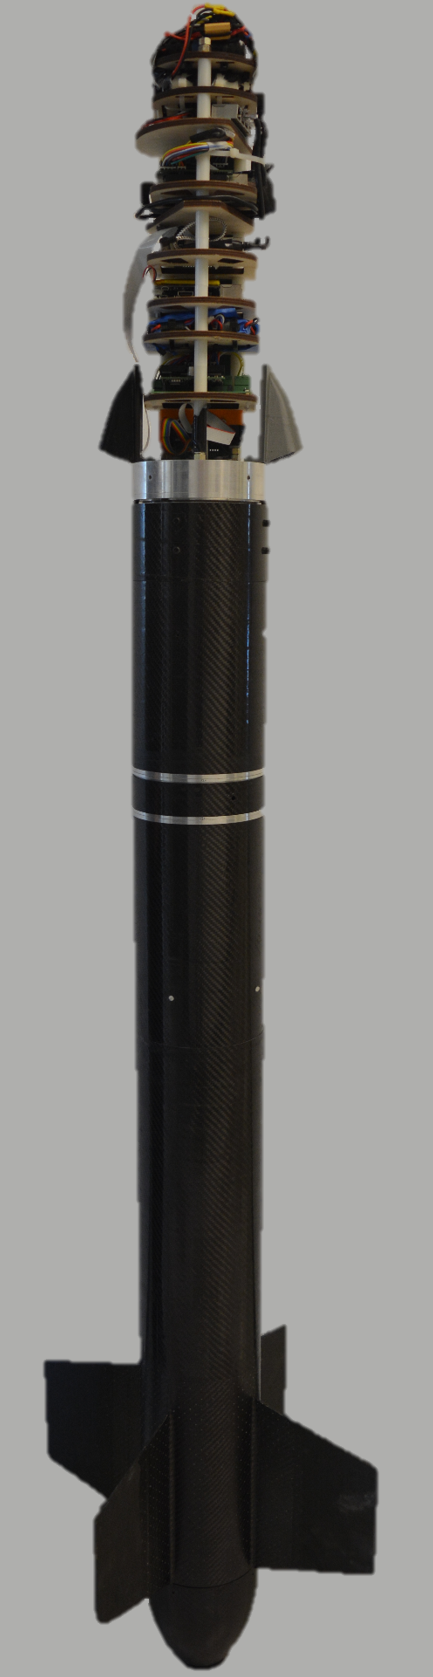
\includegraphics[width=0.37\linewidth]{09_Figures/Payload/360_final.png}
%			\caption{As Built}
%			\label{fig:360_final}
%		\end{subfigure}
%		\caption{Vehicle and Payload Launchpad Configuration}
%		\label{fig:fullVehicleAndPayloadPad}
%	\end{figure}
%	\FloatBarrier
	
	%%%%% MECHANICAL DRAWING OF SHELF STACKUP %%%%%%%%%%%%%%%%%
	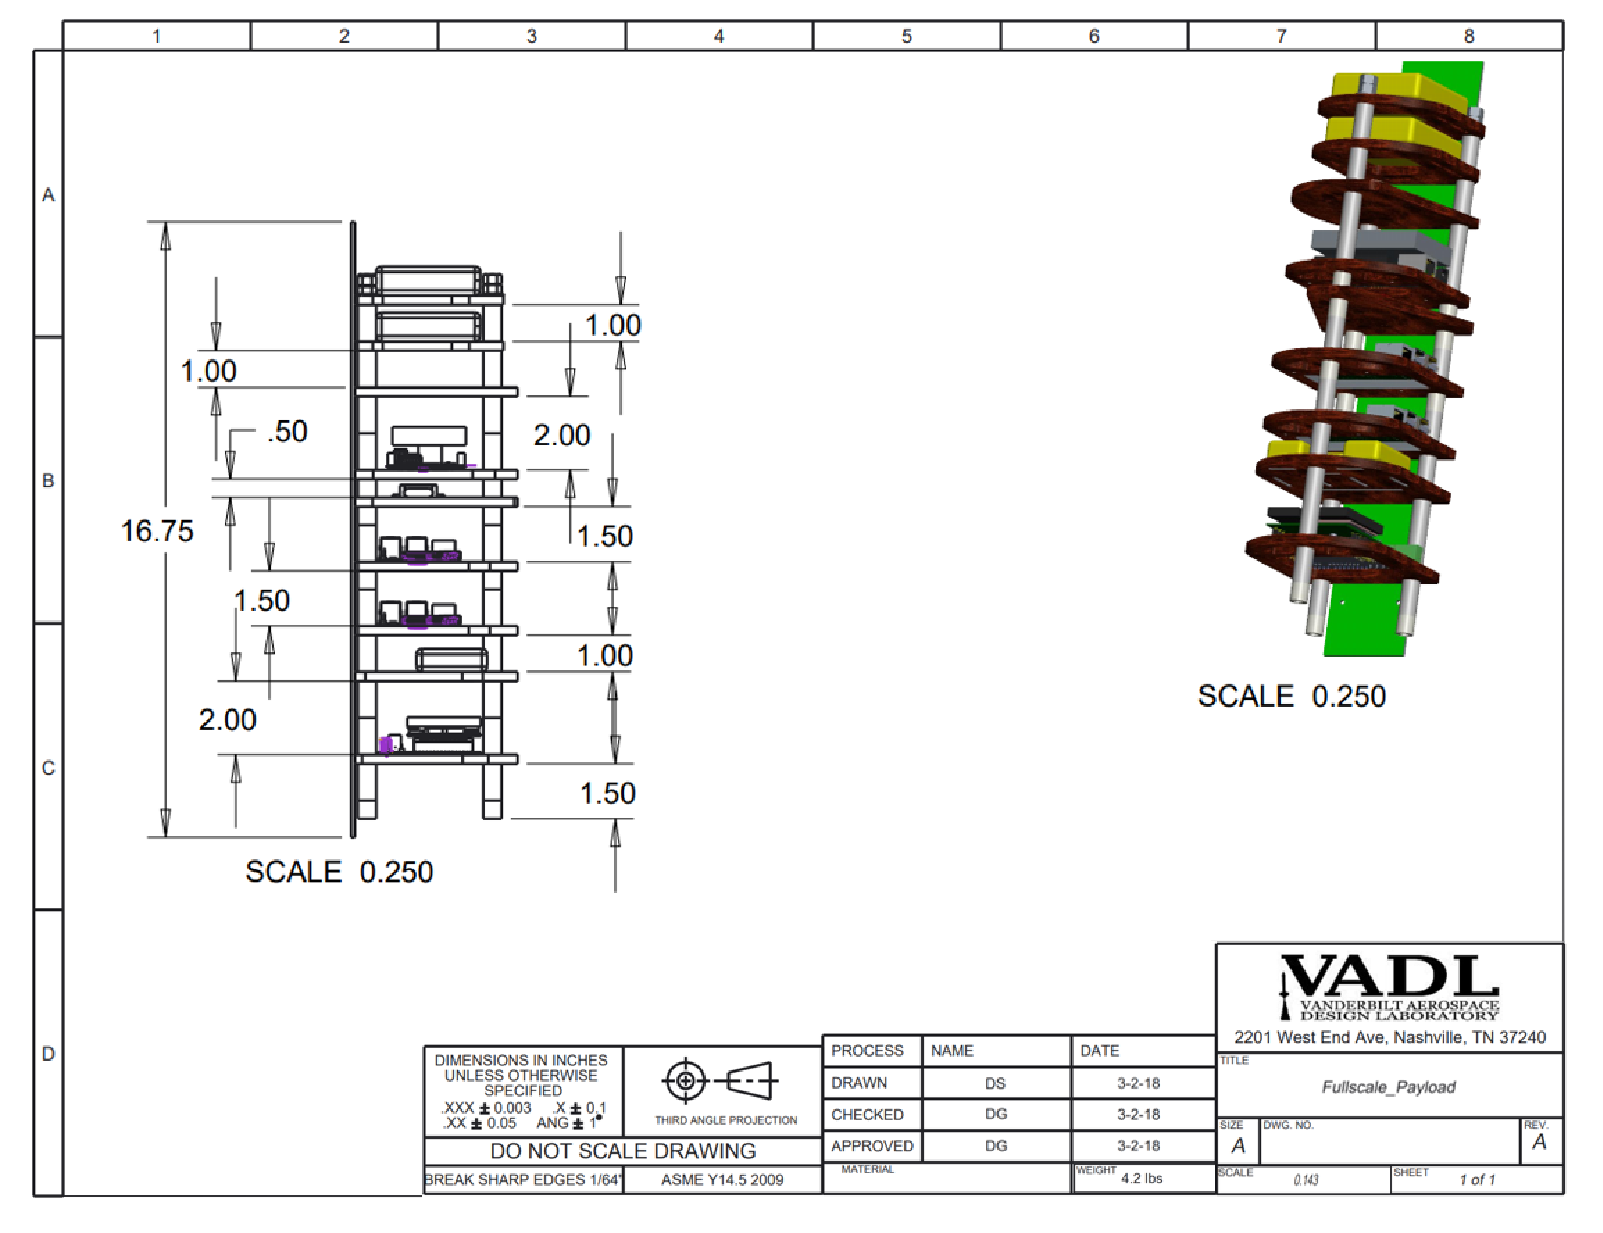
\includepdf[pages=-, pagecommand={}]{09_Figures/Payload/final_drawing1}
	
	\subsubsection{Vehicle Integration}
	
	\paragraph{Connection to SRC Mechanism}
	\label{paragraph:payload_to_src}
	The physical connection of the stepped payload to the surface of the SRC mechanism will occur using a simple threaded connection through the SRC surface with the payload's threaded rods. This surface will offer approximately 5 threads of engagement to the rods, which would most likely be more than sufficient. However, to help mitigate risk associated with vibration, jam nuts will be placed above and below that surface in order to further prevent motion along the rocket's axis. Should this prove insufficient, the threaded rods may be permanently installed using Loctite.
	
	\bigbreak
	
	\FloatBarrier{}
	\begin{figure}[!h]
		\centering
		\includegraphics[width=0.46\linewidth]{09_Figures/Payload/SRCwithShrouds.png}
		\caption{Threaded rods and camera shrouds mounted into SRC}
		\label{fig:payloadConnectSRC}
	\end{figure}
	\FloatBarrier{}
	
	% \FloatBarrier
	% \begin{figure}[!h]
	% \captionsetup[subfigure]{justification=centering}
	% \centering
	% \begin{subfigure}{.45\textwidth}
	% \centering
	% \includegraphics[width=0.4\linewidth]{09_Figures/Payload/NewSRC_w_Shrouds.jpg}
	% \caption{Threaded rods and camera shrouds mounted into SRC}
	% \label{fig:payloadConnectSRC}
	% \end{subfigure}
	% \begin{subfigure}{.45\textwidth}
	% \centering
	% \includegraphics[width=0.4\linewidth]{09_Figures/Payload/newSRCwithShrouds.png}
	% \caption{BLAH}
	% \label{fig:payloadConnectSRC_real}
	% \end{subfigure}
	% \caption{BLAH}
	% \label{fig:payloadConnect}
	% \end{figure}
	% \FloatBarrier
	
	\paragraph{Camera Shrouds}
	\label{paragraph:shroud_design}
	
	The payload requirements for this design dictate that two redundant cameras be mounted externally from the rocket, diametrically opposed. This requirement necessitates the design of aerodynamic shrouds, which simultaneously position the cameras with a maximum field of view for target detection, protect the cameras during flight, and minimally increase the drag coefficient of the rocket. Figure \ref{fig:shroudINTHEREAL} shows the shroud design.
	
	\bigbreak
	
	
	\FloatBarrier
	\begin{figure}[h]
		\centering
		\includegraphics[width=0.21\linewidth]{09_Figures/Payload/camShroud.png}
		\caption{3D-printed Camera Shroud}
		\label{fig:shroudINTHEREAL}
	\end{figure}
	\FloatBarrier
	
	The payload cameras are housed by aerodynamic shrouds mounted directly on the SRC mechanism. The shrouds are each affixed by two 6-32 screws, and designed to align on the outer edge of the SRC mechanism. The carbon fiber body will slide over the shrouds and be bolted to the SRC mechanism.
	
	
	\bigbreak
	The camera shrouds are designed to allow mounting of the cameras on an angled plane internal to the camera shroud. This angle is determined by the angle of the camera's vertical field of view, maximizing the field of view of the cameras. The cameras will be bolted to the plane using 4 threaded aluminum 2-56 bolts and nuts.
	
	\bigbreak
	
\end{document}
